% Nội dung: chaptersnew/chapter01 (1).tex; trình bày theo các layout trong chapters/.
\section{Chương 1: Giới thiệu eBPF}
\ChapterDivider{Chương 1}{Giới thiệu eBPF}{Từ nhu cầu quan sát Linux đến công nghệ eBPF}

\begin{frame}{Container này có đang được sử dụng?}
  \small
  Một hệ thống tính toán dùng chung có thể chạy mỗi phiên làm việc trong một container.
  Mức sử dụng CPU thấp có thể xuất hiện ngay cả khi container đang tải dữ liệu.
  \vspace{0.35cm}
  \begin{columns}[c,onlytextwidth]
    \begin{column}{0.47\textwidth}
      \begin{block}{Hoạt động cần quan sát (I/O)}
        \begin{itemize}
          \item Có đang đọc hoặc ghi dữ liệu?
          \item Có đang gửi hoặc nhận dữ liệu qua mạng?
          \item Có đang nhập gì không? Hay chỉ đang dùng để đọc tài liệu?
        \end{itemize}
      \end{block}
    \end{column}
    \begin{column}{0.49\textwidth}
      \centering
      \textbf{Ví dụ: đang tải một bộ dữ liệu}\par\medskip
      \begin{tikzpicture}
        \node[ebpfuser, text width=2.3cm, minimum height=1.0cm] (network)
        {Nhận dữ liệu\\qua mạng};
        \node[ebpfuser, text width=2.3cm, minimum height=1.0cm, right=0.7cm of network] (disk)
        {Ghi dữ liệu\\xuống đĩa};
        \draw[arr] (network) -- (disk);
      \end{tikzpicture}
    \end{column}
  \end{columns}
  \vspace{0.35cm}
  \centering\textbf{Trước khi thu hồi tài nguyên, làm sao biết từng container\\
    còn đọc, ghi hoặc truyền dữ liệu qua mạng?}
  \note{Ví dụ giả định. CPU và I/O là các tín hiệu bổ sung cho nhau khi đánh giá hoạt động của container.}
\end{frame}

\begin{frame}{Các phương pháp truyền thống}
  \begin{columns}[T,onlytextwidth]
    \begin{column}{0.48\textwidth}
      \begin{block}{Application logging}
        Ứng dụng chủ động ghi sự kiện.\\
        Log mới có thể đòi hỏi thay đổi mã ứng dụng.
      \end{block}
      \begin{block}{\texttt{strace}}
        Theo dõi system calls và tương tác tiến trình với kernel.
      \end{block}
    \end{column}
    \begin{column}{0.48\textwidth}
      \begin{block}{\texttt{perf}}
        Thu thập, phân tích hoạt động và hiệu năng.\\
        Lấy mẫu, chi phí tùy phép đo.
      \end{block}
      \begin{block}{Kernel module}
        Mở rộng kernel bằng mã đặc quyền cao.\\
        Lỗi có thể ảnh hưởng toàn hệ thống.
      \end{block}
    \end{column}
  \end{columns}
  \vspace{0.20cm}
  Trong phép so sánh tiếp theo, \texttt{perf trace} xuất từng lượt đọc để script tổng hợp.
  Chương trình eBPF có thể tính cùng chỉ số ngay trong kernel.
\end{frame}

\begin{frame}{eBPF mở rộng khả năng của Linux kernel}
  \small
  \centering
  \renewcommand{\arraystretch}{1.45}
  \begin{tabular}{@{}L{0.44\textwidth}L{0.48\textwidth}@{}}
    \toprule
    \textbf{Mã nguồn kernel và kernel module} & \textbf{Chương trình eBPF} \\
    \midrule
    Mã nguồn kernel sửa đổi có thể cần build và khởi động lại.
      & BPF API nạp chương trình vào kernel đang chạy. \\
    Kernel module có quyền truy cập rộng. Lỗi có thể ảnh hưởng toàn hệ thống.
      & Verifier kiểm tra chương trình khi nạp. Phạm vi thực thi phụ thuộc program type và hook. \\
    \bottomrule
  \end{tabular}

  \medskip
  \textbf{Ví dụ.} Một tracepoint tại \texttt{openat()} cho phép đếm yêu cầu mở tệp ngay trên host.

  \smallskip
  {\scriptsize Nguồn \href{https://ebpf.io/what-is-ebpf/}{eBPF.io}}
  \note{Khoảng 1 phút. eBPF đưa logic xử lý sự kiện vào các điểm kernel hỗ trợ. Bộ đếm mở tệp chạy mà không cần thay đổi mã ứng dụng hoặc khởi động lại máy. Sửa kernel và kernel module vẫn phục vụ các nhu cầu rộng hơn. Phép thử đọc chậm cho thấy khác biệt khi việc tổng hợp diễn ra trong kernel.}
\end{frame}

\begin{frame}{Phép thử đếm lượt đọc chậm theo container}
  \small
  Hai container đang chạy cùng một chương trình. Mỗi bên thực hiện \textbf{20 lượt đọc}.
  Container B được cấp dữ liệu trễ khoảng 320 ms ở bốn lượt.
  \vspace{0.25cm}
  \begin{columns}[T,onlytextwidth]
    \begin{column}{0.48\textwidth}
      \begin{block}{\texttt{perf trace} + script}
        Kernel ghi nhận từng lượt đọc.\\[0.15cm]
        $\downarrow$ Từng bản ghi đi ra ngoài kernel.\\[0.15cm]
        Script lọc lượt trên 200 ms và đếm.
      \end{block}
    \end{column}
    \begin{column}{0.48\textwidth}
      \begin{block}{eBPF + bộ đếm}
        Probe đo từng lượt đọc ngay trong kernel.\\[0.15cm]
        Probe lọc lượt trên 200 ms và đếm.\\[0.15cm]
        $\downarrow$ Công cụ giám sát lấy số tổng sau 5 giây.
      \end{block}
    \end{column}
  \end{columns}
  \vspace{0.30cm}
  \centering\textbf{Hai cách cho cùng số lượt đọc chậm? Bao nhiêu dữ liệu đi ra ngoài kernel?}
\end{frame}

\begin{frame}{Kết quả đo lượt đọc chậm theo container}
  \small
  \begin{columns}[c,onlytextwidth]
    \begin{column}{0.68\textwidth}
      \centering
      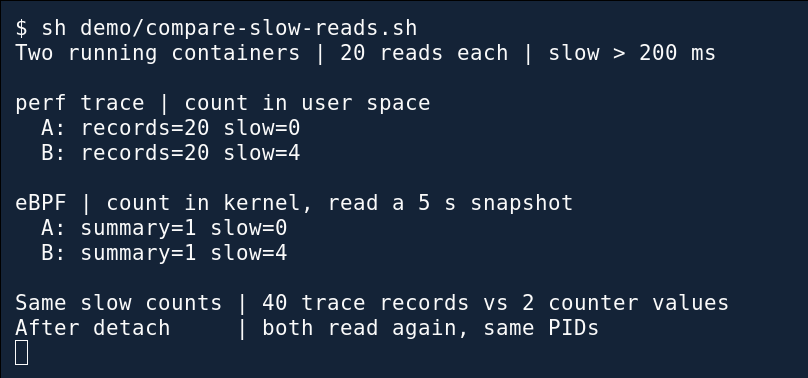
\includegraphics[width=\linewidth]{images/demo-slow-reads-terminal.png}
    \end{column}
    \begin{column}{0.30\textwidth}
      \begin{block}{Cùng kết quả}
        A có \textbf{0}, B có \textbf{4} lượt đọc chậm.
      \end{block}
      \begin{block}{Dữ liệu nhận được}
        \texttt{perf trace}: \textbf{40} bản ghi.\\
        eBPF: \textbf{2} giá trị tổng.
      \end{block}
    \end{column}
  \end{columns}
  \vspace{0.22cm}
  \centering\textbf{Sau khi gỡ probe, cả hai tiến trình đọc tiếp với cùng PID.}
  \note{Ảnh từ terminal khi chạy demo thật. 40 là số bản ghi của các lượt đọc mẫu mà script perf xử lý. 2 là số giá trị tổng theo container ở lần đọc map đầu tiên. Phép đo không đếm các gói nội bộ hay đo CPU.}
\end{frame}

\begin{frame}[fragile]{Phép đo eBPF trên kernel đang chạy}
  \small
  Hai tracepoint tại đầu và cuối \texttt{read()} cung cấp mốc thời gian cho phép đo.
  \vspace{0.20cm}
  \begin{columns}[T,onlytextwidth]
    \begin{column}{0.43\textwidth}
      \begin{block}{Lọc và đếm bên ngoài kernel}
        \begin{lstlisting}
perf trace -a -G "$path_a" -e read
\end{lstlisting}
        Script đọc thời lượng từ từng dòng trace rồi đếm các lượt trên 200 ms.
      \end{block}
    \end{column}
    \begin{column}{0.52\textwidth}
      \begin{block}{Lọc và đếm trong kernel}
        \lstinputlisting[firstline=17,lastline=19]{demo/slow-reads.bt}
        Probe cộng vào bộ đếm của container. Sau 5 giây, công cụ giám sát đọc số tổng.
      \end{block}
    \end{column}
  \end{columns}
  \vspace{0.30cm}
  \begin{center}
    \textbf{Phép đo có thể bắt đầu và kết thúc trong khi máy chủ\\
      tiếp tục phục vụ các container.}
  \end{center}
  \note{Trích mã thực thi. Probe được kernel kiểm tra khi nạp và cần hook cùng quyền phù hợp. Bản đầy đủ lưu thời điểm bắt đầu theo TID và xóa trạng thái khi lượt đọc kết thúc.}
\end{frame}
